\documentclass[14pt]{extarticle}
\usepackage[utf8]{inputenc}
\usepackage{amsmath}
\usepackage{amsfonts}
\usepackage{graphicx}
\usepackage{setspace}
\usepackage{geometry}
\usepackage{enumitem}
\usepackage{amssymb}
\usepackage{xcolor}
\usepackage{mathtools}
\usepackage{float}
\usepackage{listings}

\geometry{
    top=1in,
    bottom=1in,
    left=1in,
    right=1in,
    headheight=14pt,
    headsep=25pt,
    footskip=30pt
}

\title{Bayes Theorem}
\author{Yana Jin}
\date{Wednesday, 19th September 2024}

\onehalfspacing

\pagenumbering{gobble}

\begin{document}

\subsection*{Galton, Pearson, and the Peas: A Brief History of Linear Regression (and correlation)}

\noindent
\textbf{Sir Francis Galton}\\
 - Worked on inherited characteristics of sweet peas\\
 - Originally conceived modern notions of regression and correlation\\
 - Cousin of Charles Darwin\\
 - Was interested in how strongly characteristics of one generation of living things manifested in the following generation\\
 - Chose sweet peas because this species could self fertilize\\
 - Eliminated genetic contributions from multiple sources\\
\begin{figure}[H]
    \centering
    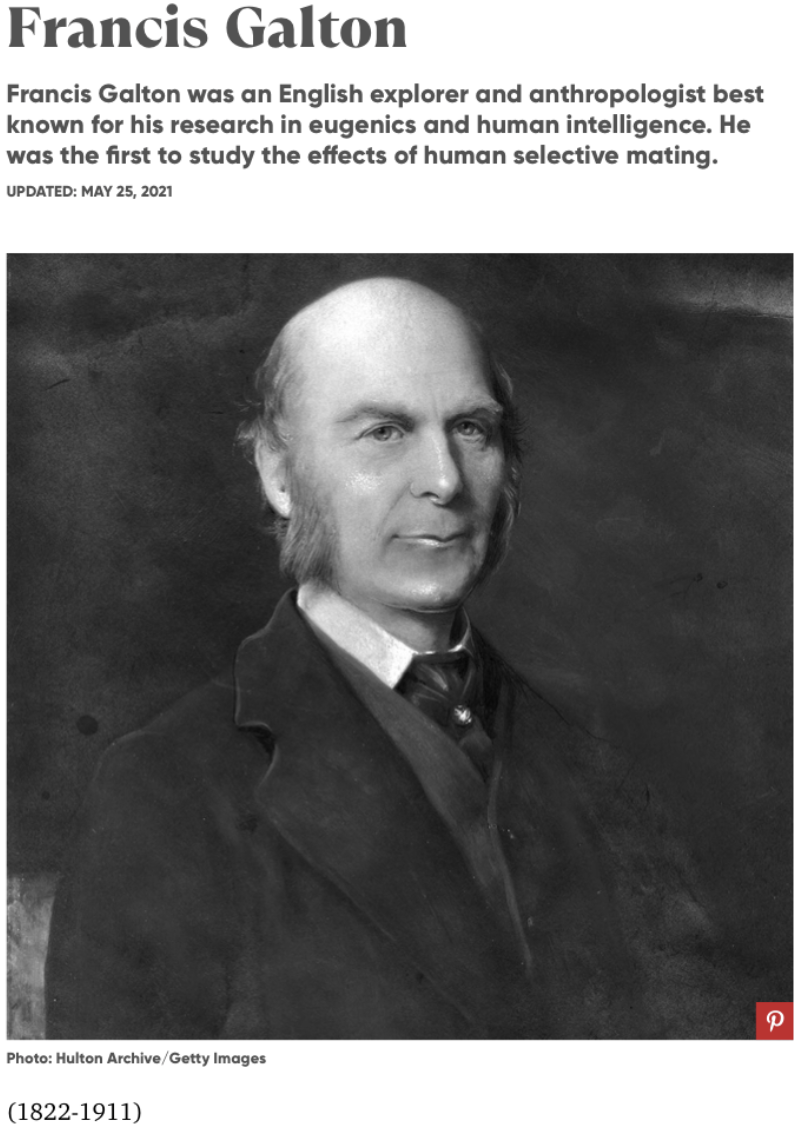
\includegraphics[width=0.45\textwidth]{fig1.png}
\end{figure}
\[\text{Source: biography.com}\]

\begin{figure}[H]
    \centering
    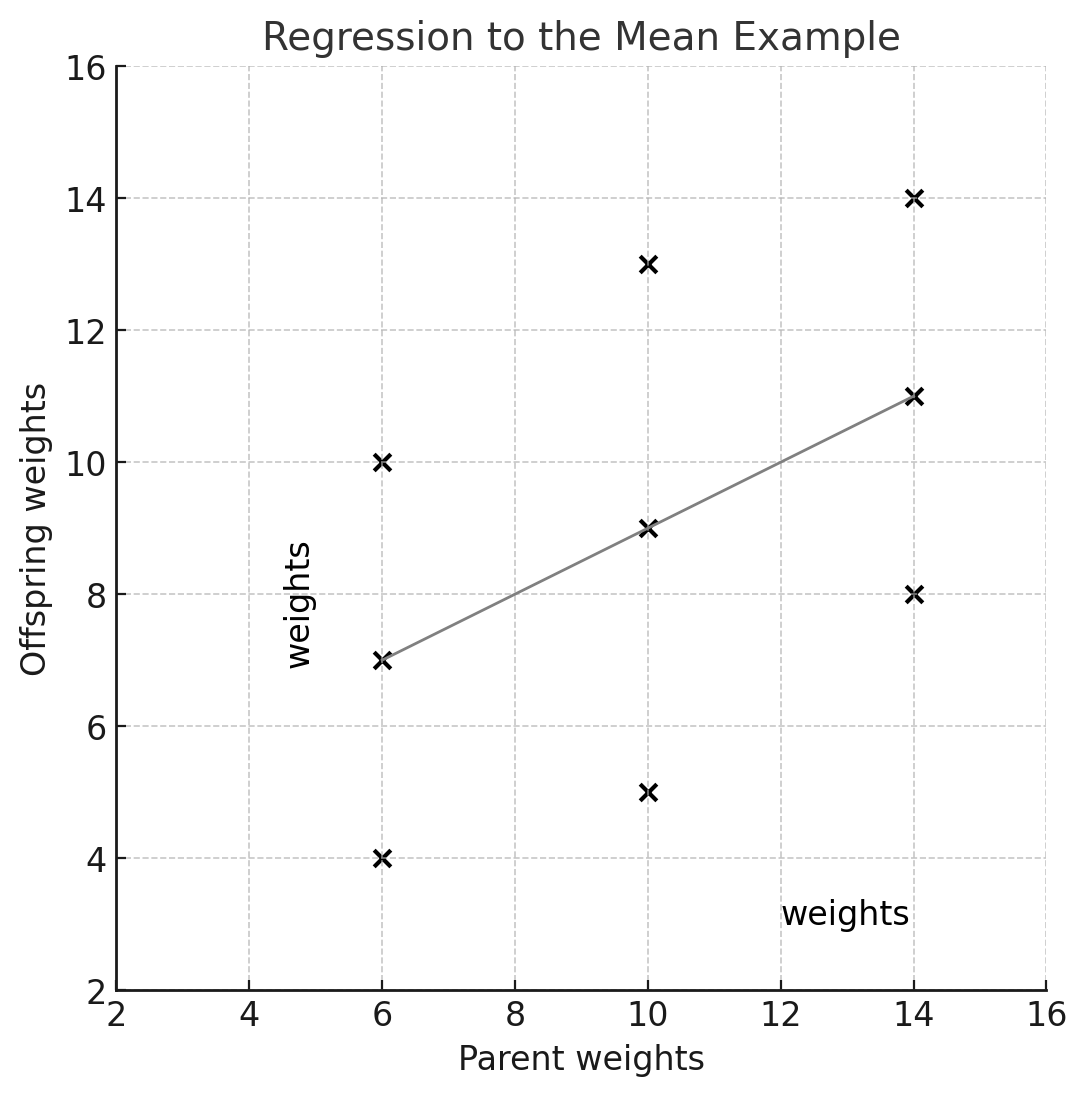
\includegraphics[width=0.8\textwidth]{fig2.png}
\end{figure}

\noindent \textbf{Explanation of the graph:} \\
\noindent \textcolor{green}{- Regression to the mean (Y values closer to $\bar{Y}$ than X values are to $\bar{X}$)}\\
\noindent \textcolor{blue}{- Approx. equal variability in Y values at a given X value}\\
\noindent \textcolor{red}{- Median weights of the daughter seeds from a particular size of mother approx. described straight line with slope $<$ 1.0} \\
\noindent \textcolor{blue}{- Made up data}

\noindent
$\Rightarrow$ because slope $< 1.0$, Galton concluded there was a regression to the mean for that generation of peas.\\

\noindent
Above figure shows line connecting the means of the columns of data points, which indicates the degree of regression to the mean.

\subsection*{Galton's Recognition of the Generality of Regression Slope}

\noindent
Galton generalized his work to a variety of heredity problems:\\
 - temperament \\
 - artistic ability\\
 - disease incidence

\noindent
\textbf{His important breakthrough:} \\
If degree of association between two variables held constant, then slope of the regression line could be described if variability of two variables were known.

\begin{figure}[H]
    \centering
    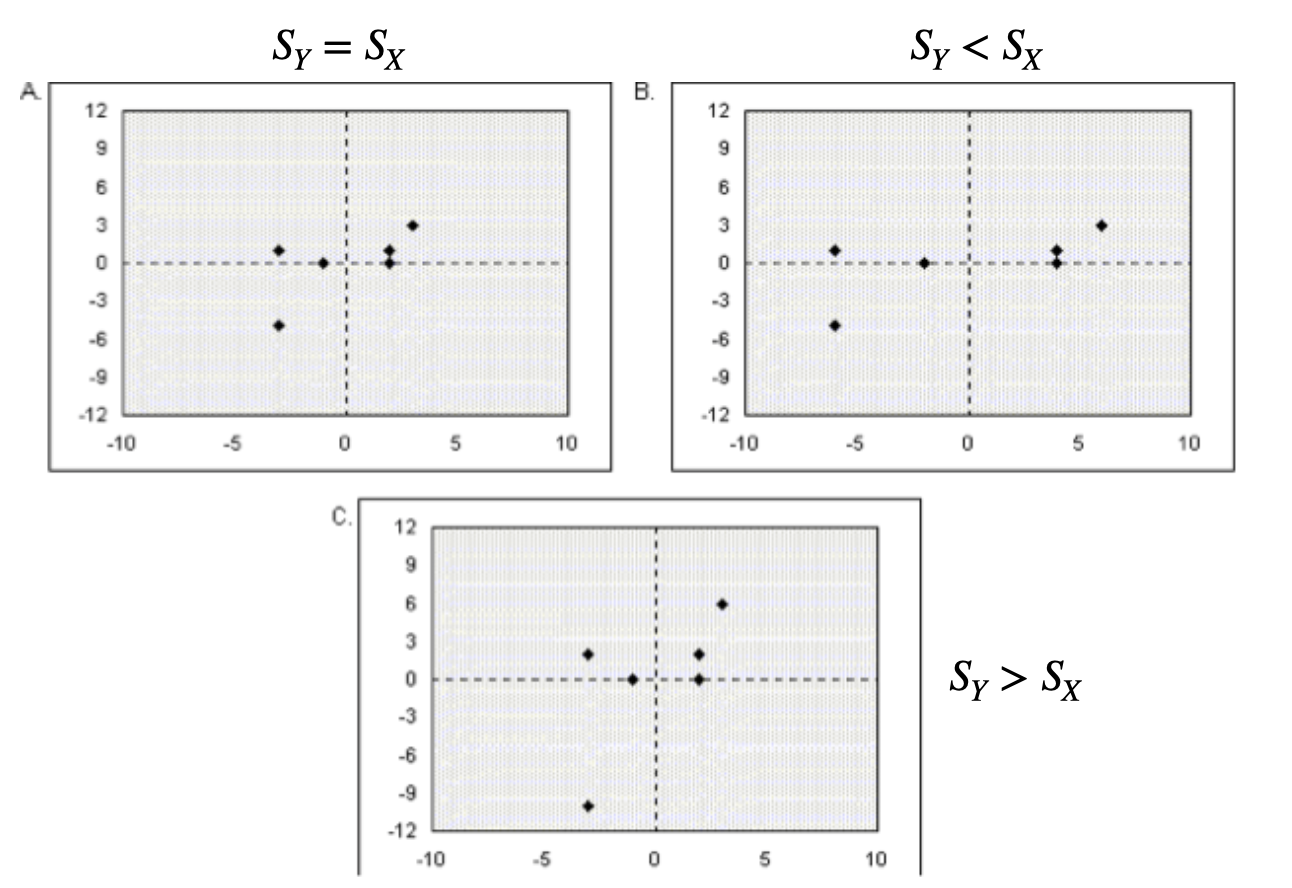
\includegraphics[width=0.9\textwidth]{fig3.png}
\end{figure}

\noindent
$(r = 0.64 \text{ for all figures})$\\
\noindent
Slope of line $\uparrow$ as $S_Y > S_X$.\\
\noindent
Galton had recognized the rudimentary regression equation:
\[
\textcolor{red}{y = r\left(\frac{S_Y}{S_X}\right)x}
\]

\subsection*{Pearson's Mathematical Development of Correlation and Regression}

\noindent
In 1896, Pearson published the first rigorous treatment of correlation and regression.

\noindent
Pearson demonstrated that optimum values $\textcolor{red}{\sum_{i} (y_i - \hat{y_i})^2 \quad \text{(smallest)}}
$ for regression slope and correlation coefficient could be calculated using product-moment:
\[
\frac{\sum_{i} X_i Y_i}{n}
\]

\noindent
Here $x_i$ and $y_i$ are actually deviations from their respective means.

\begin{figure}[H]
    \centering
    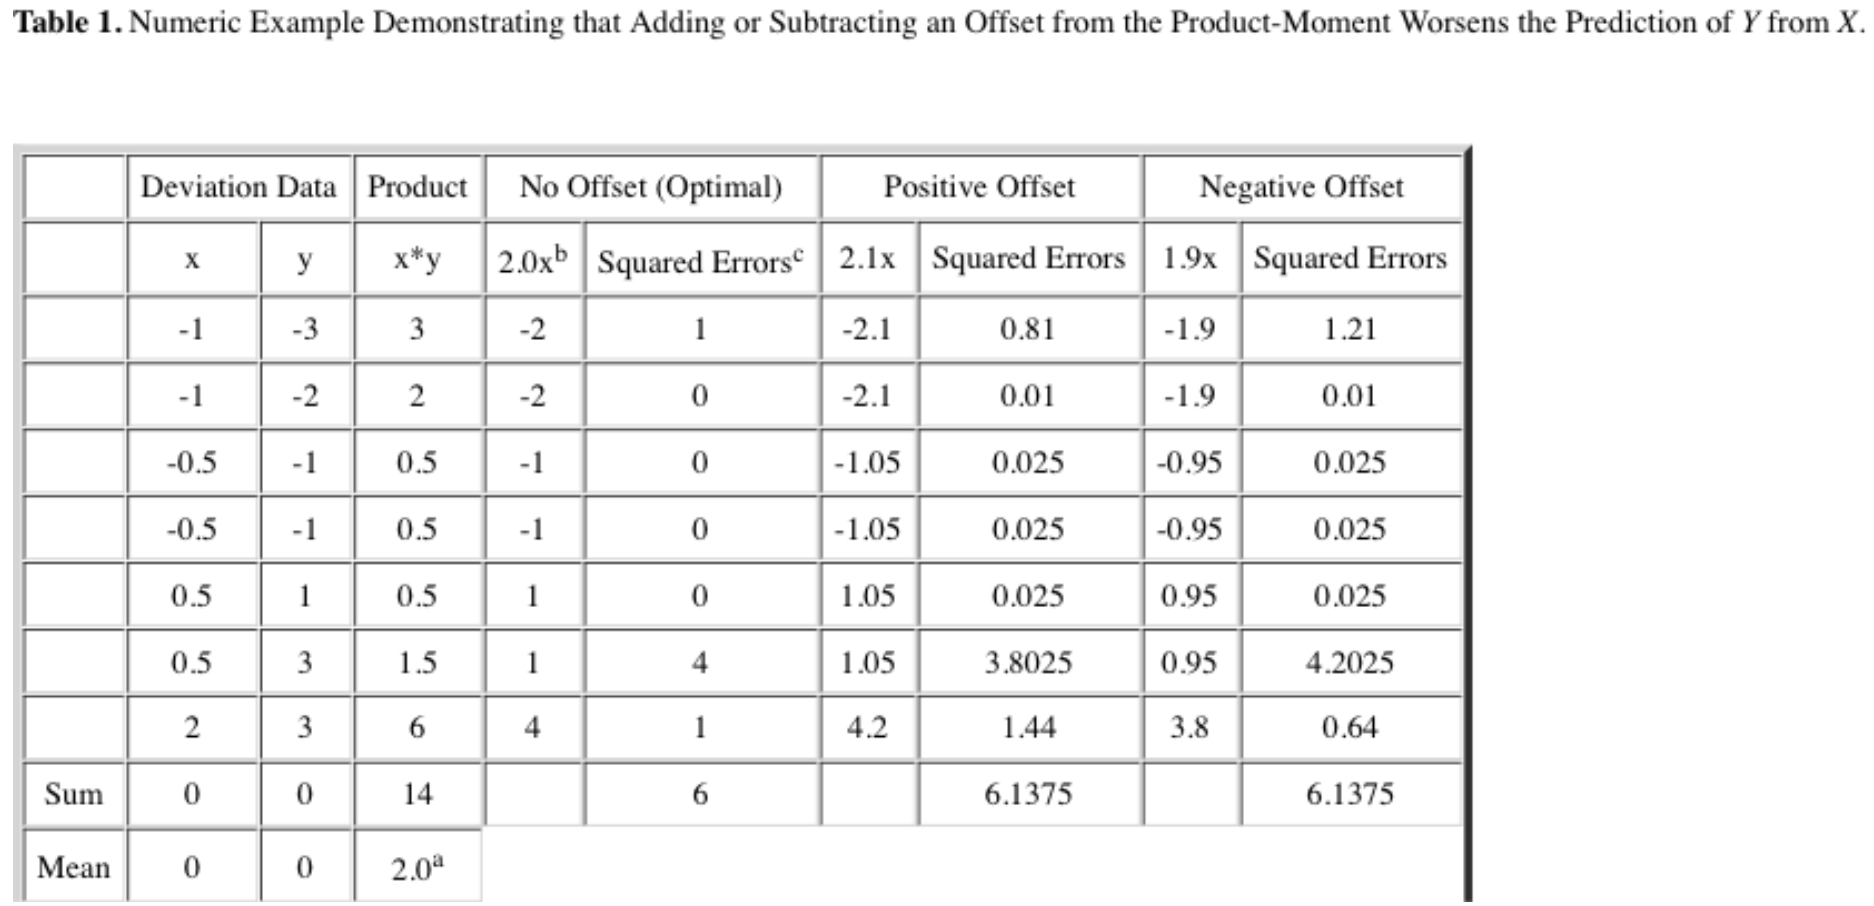
\includegraphics[width=1\textwidth]{fig4.png}
\end{figure}

\newpage

\section*{Testing Population $\rho$}
\noindent
Suppose interested in testing the following hypotheses:
\[
H_0: \rho = 0
\]
\[
H_1: \rho \neq 0
\]
\noindent
Fact: 
\[
t(X, Y) = \frac{r(XY)\sqrt{n-2}}{\sqrt{1 - r(XY)^2}} \quad \overset{H_0}{\sim} t_{n-2} 
\]

\noindent
Reject $H_0$ at level $\alpha$ if:
\[
|t_{\text{obs}}| > t_{1-\alpha/2, n-2}
\]
\textcolor{red}{\quad ($t_{obs}$: observed value from sample)}

\noindent
A one-tailed test for a positive correlation between $X$ and $Y$ tests:
\[
H_0: \text{when } X \uparrow \text{ does } Y \uparrow \text{ in the population?}
\]
\section*{Confidence Intervals for $\rho$}

\noindent
We use Fisher's $Z$ transform:

\[
Z = \frac{1}{2} \log_e \left( \frac{1 + r(XY)}{1 - r(XY)} \right)
\]

\noindent
For large $n$, this is distributed under $H_0$ as:

\[
N(0, \left( \frac{1}{\sqrt{n - 3}} \right)^2)
\]

\noindent $\therefore$ First, find $100 \times (1-\alpha) \%$ CI based on $Z$ and then transform back to the $r(XY)$ scale.

\noindent
\textbf{How?}
\[
Z = \frac{1}{2} \log_e \left( \frac{1 + r}{1 - r} \right)
\]
\[
2 \cdot Z = \log_e \left( \frac{1 + r}{1 - r} \right)
\]
\[
\exp(2Z) = \frac{1 + r}{1 - r}
\]
\[
\exp(2Z)(1 - r) = 1 + r
\]
\[
\exp(2Z) - r \exp(2Z) = 1 + r
\]
\[
\exp(2Z) - 1 = r(\exp(2Z) + 1)
\]
\[
\Rightarrow r = \frac{\exp(2Z) - 1}{\exp(2Z) + 1}
\]

\noindent
\textbf{Example}

\noindent
Pearson's sample $r$ for a study investigating the association of basal metabolic rate with total energy expenditure was estimated as 0.7283 in $n=13$ women. Derive a 95\% CI for $\rho$.
\[
Z = \frac{1}{2} \log_e \left( \frac{1 + 0.7283}{1 - 0.7283} \right) = 0.9251
\]
\noindent
Lower limit of 95\% CI:
\[
0.9251 - 1.96 \left( \frac{1}{\sqrt{13 - 3}} \right) = 0.3053
\]

\noindent
Upper limit of 95\% CI:
\[
0.9251 + 1.96 \left( \frac{1}{\sqrt{13 - 3}} \right) = 1.545
\]
\noindent
Now transform back to the $r$ scale:

\noindent
$\therefore$ the 95\% confidence interval for $\rho$ is:
\[
\left( \frac{\exp(2 \times 0.3053) - 1}{\exp(2 \times 0.3053) + 1}, \frac{\exp(2 \times 1.545) - 1}{\exp(2 \times 1.545) + 1} \right)
\]
\[
= (0.30, 0.91)
\]



\end{document}